\documentclass[12pt]{extarticle}
\title{}
\author{}
\date{}
\usepackage[shortlabels]{enumitem}


%paper setup
\usepackage{geometry}
\geometry{letterpaper, portrait, margin=1in}
\usepackage{fancyhdr}
% sans serif font:
\usepackage{cmbright}
%symbols
\usepackage{amsmath}
\usepackage{bigints}
\usepackage{amssymb}
\usepackage{amsthm}
\usepackage{mathtools}
\usepackage{bbold}
\usepackage[hidelinks]{hyperref}
\usepackage{gensymb}
\usepackage{multirow,array}
\usepackage{multicol}

\newtheorem*{remark}{Remark}
\usepackage[T1]{fontenc}
\usepackage[utf8]{inputenc}

%chemistry stuff
%\usepackage[version=4]{mhchem}
%\usepackage{chemfig}

%plotting
\usepackage{pgfplots}
\usepackage{tikz}
\usetikzlibrary{cd}
\tikzset{middleweight/.style={pos = 0.5}}
%\tikzset{weight/.style={pos = 0.5, fill = white}}
%\tikzset{lateweight/.style={pos = 0.75, fill = white}}
%\tikzset{earlyweight/.style={pos = 0.25, fill=white}}

%\usepackage{natbib}

%graphics stuff
\usepackage{graphicx}
\graphicspath{ {./images/} }
%\usepackage[style=numeric, backend=biber]{biblatex} % Use the numeric style for Vancouver
%\addbibresource{the_bibliography.bib}
%code stuff
%when using minted, make sure to add the -shell-escape flag
%you can use lstlisting if you don't want to use minted
%\usepackage{minted}
%\usemintedstyle{pastie}
%\newminted[javacode]{java}{frame=lines,framesep=2mm,linenos=true,fontsize=\footnotesize,tabsize=3,autogobble,}
%\newminted[cppcode]{cpp}{frame=lines,framesep=2mm,linenos=true,fontsize=\footnotesize,tabsize=3,autogobble,}

%\usepackage{listings}
%\usepackage{color}
%\definecolor{dkgreen}{rgb}{0,0.6,0}
%\definecolor{gray}{rgb}{0.5,0.5,0.5}
%\definecolor{mauve}{rgb}{0.58,0,0.82}
%
%\lstset{frame=tb,
%	language=Java,
%	aboveskip=3mm,
%	belowskip=3mm,
%	showstringspaces=false,
%	columns=flexible,
%	basicstyle={\small\ttfamily},
%	numbers=none,
%	numberstyle=\tiny\color{gray},
%	keywordstyle=\color{blue},
%	commentstyle=\color{dkgreen},
%	stringstyle=\color{mauve},
%	breaklines=true,
%	breakatwhitespace=true,
%	tabsize=3
%}
% text + color boxes
%\renewcommand{\mathbf}[1]{\mathbb{#1}}
%\usepackage[most]{tcolorbox}
%\tcbuselibrary{breakable}
%\tcbuselibrary{skins}
%\newtcolorbox{problem}[1]{colback=white,enhanced,title={\small #1},
%          attach boxed title to top center=
%{yshift=-\tcboxedtitleheight/2},
%boxed title style={size=small,colback=black!60!white}, sharp corners, breakable}
%including PDFs
%\usepackage{pdfpages}
\setlength{\parindent}{0pt}
\usepackage{cancel}
\pagestyle{fancy}
\fancyhf{}
\rhead{Avinash Iyer}
\lhead{Economics of Education: Problem Set 3}
\newcommand{\card}{\text{card}}
\newcommand{\ran}{\text{ran}}
\newcommand{\N}{\mathbb{N}}
\newcommand{\Q}{\mathbb{Q}}
\newcommand{\Z}{\mathbb{Z}}
\newcommand{\R}{\mathbb{R}}
\newcommand{\C}{\mathbb{C}}
\newcommand{\iprod}[2]{\left\langle #1,#2\right\rangle}
\newcommand{\norm}[1]{\left\Vert #1\right\Vert}
\setcounter{secnumdepth}{0}
\begin{document}
  \section{Primary School Funding}%
  While listening to the article, I was not particularly shocked at the dynamics of relatively high education spending while also having relatively little to show for it (in the form of amenities for students). The costs of operating a school and paying for teachers is extremely high, especially in the modern era due to the abundance of outside options that educated women have in the labor market. While the Roy model would predict that the higher earnings for college-educated women in outside options would result in lower teacher wages/skill, but there are likely countervailing forces at play that bring the compensation of teachers in relative alignment with the compensation of other college-educated professions, such as increased labor market competition. The result of school funding being relatively confined to the basics of running the school mean that it's likely that fewer field trips/extracurricular activities are funded as the cost of teacher labor and school maintenance increase.
  \section{Student Accountability}%
  Steven Levitt, in the Freakonomics episode about incentives, effectively discusses how children (relative to adults) are very present-oriented (i.e., they have a very large discount factor). Qua Levitt, younger children are especially more responsive towards incentives of any kind than older children, who have a higher threshold before they start to respond to the incentive for performance; and that this effect is more effective for boys than girls. Specifically, I think that the realm Levitt is describing is one that is much less abstract than the incentives seen at play in the NY Times article, which discusses less how to get children to do their homework and is focused more on them trying and failing before they learn to do their homework. The NY Times approach was something my parents did --- they did not tell me to do my homework, nor did they even help me with remembering what homework I had, they just threw me in the deep end to fend for myself. I can't say it turned out perfect (after all, I am submitting this homework assignment way later than when I could have had it done), but it did provide me much better setup, compared to the anecdotal evidence Levitt brings towards his college experience, for consistently dealing with a situation where one has to be extremely self-motivated to get homework done.
  \section{Teacher Labor Markets}%
  \begin{enumerate}[(a)]
    \item We see that teacher wage and skill level rise as a result of a higher $\alpha_T$.
      \begin{center}
        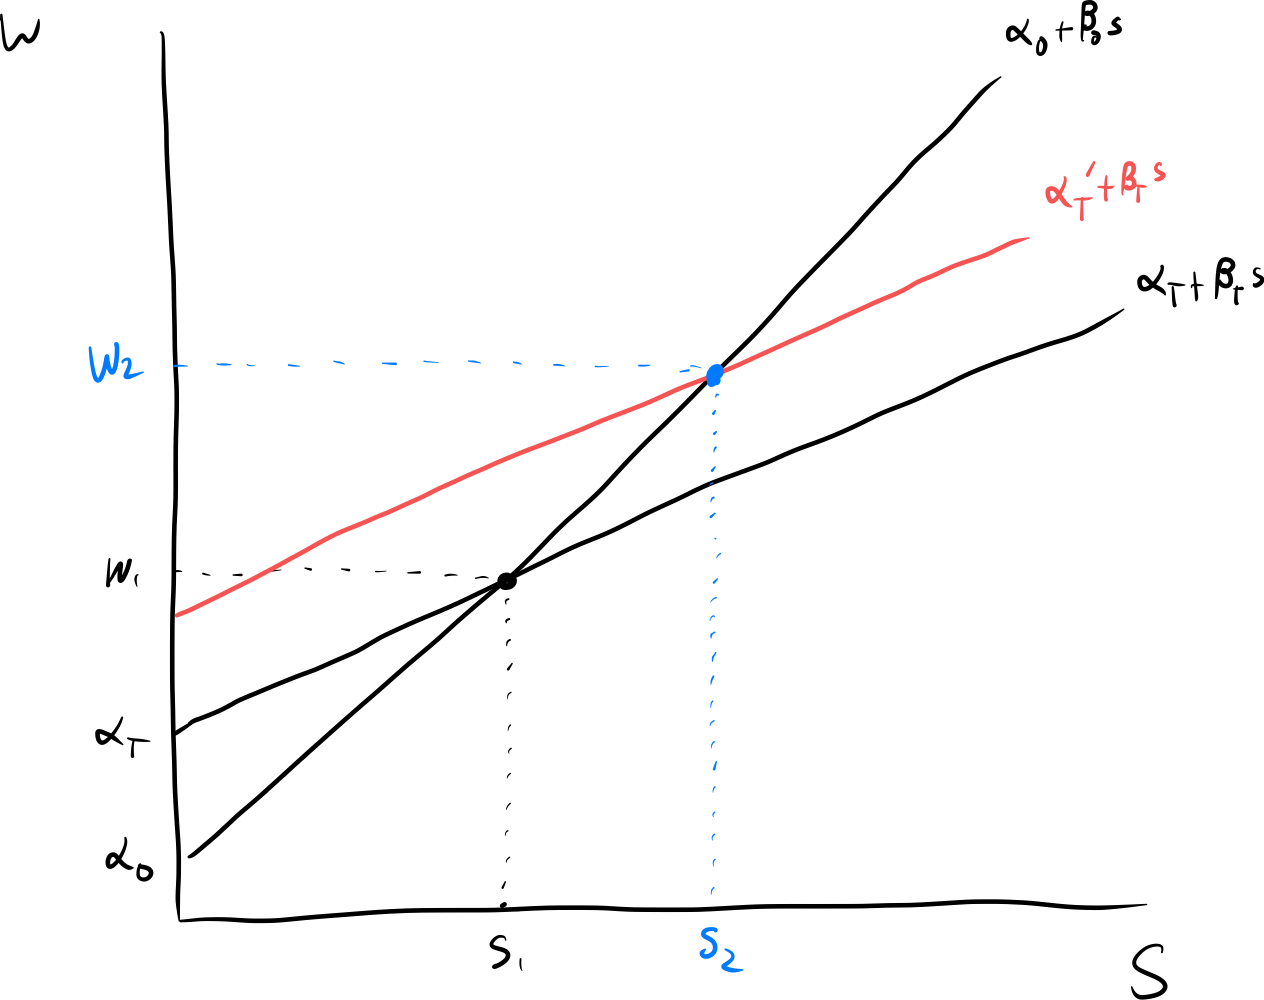
\includegraphics[width=10cm]{images/ps3q3a.png}
      \end{center}
    \item The duty-to-bargain provisions yield lower returns to skill and a flatter wage structure, meaning that the direction of skill and wage changes are ambiguous (in this case, we have drawn a reduction in skill and wage)
      \begin{center}
        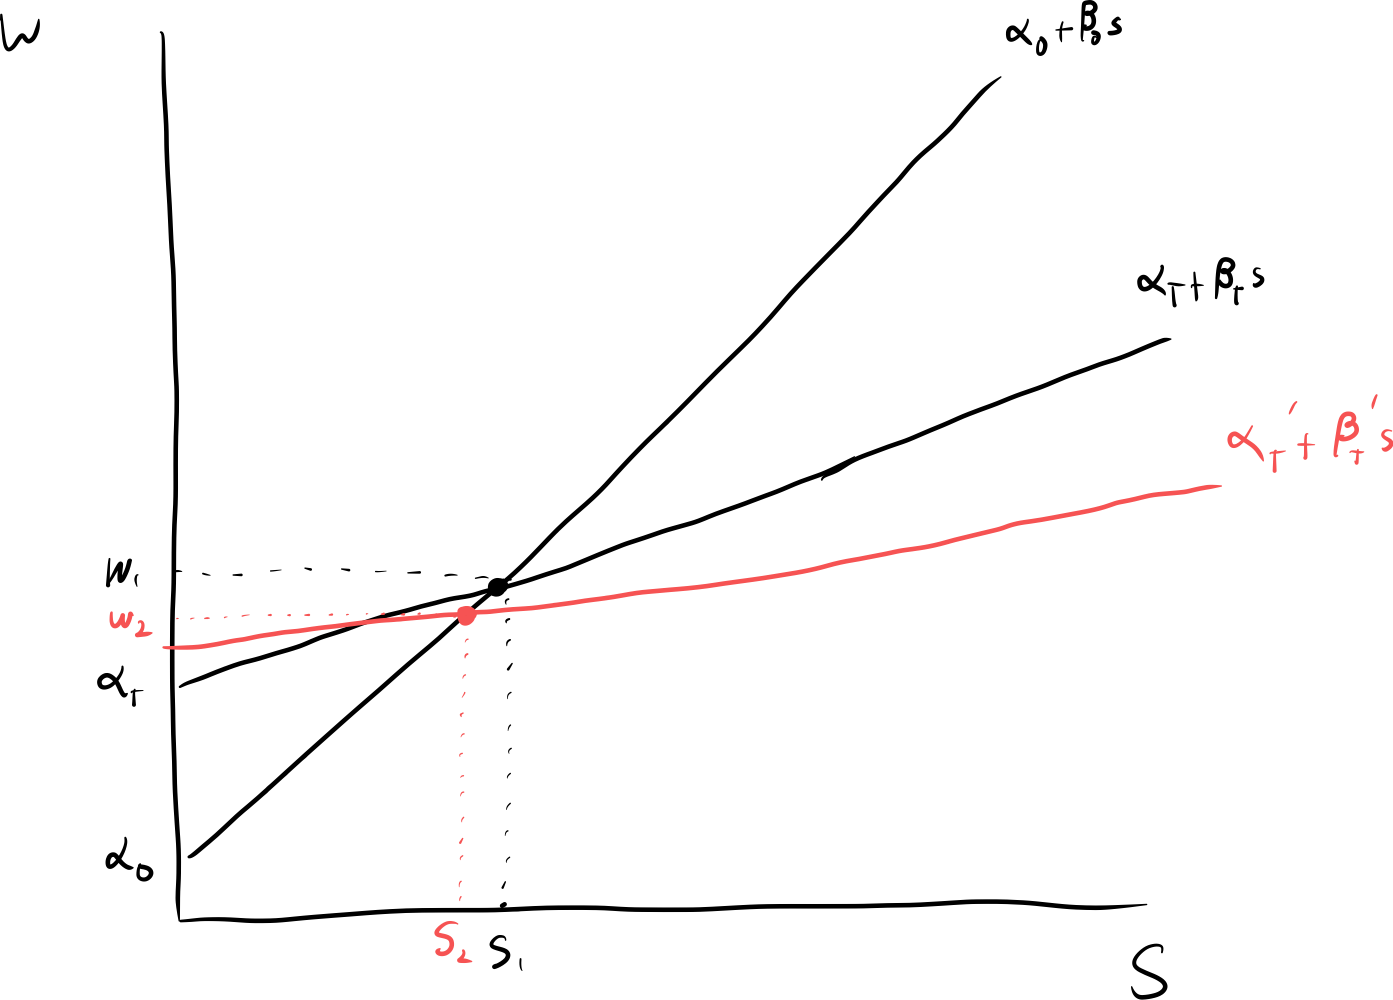
\includegraphics[width=10cm]{images/ps3q3b.png}
      \end{center}
    \item The accountability system increases return to skill, reducing $\alpha_T$ and increasing $\beta_T$.
      \begin{center}
        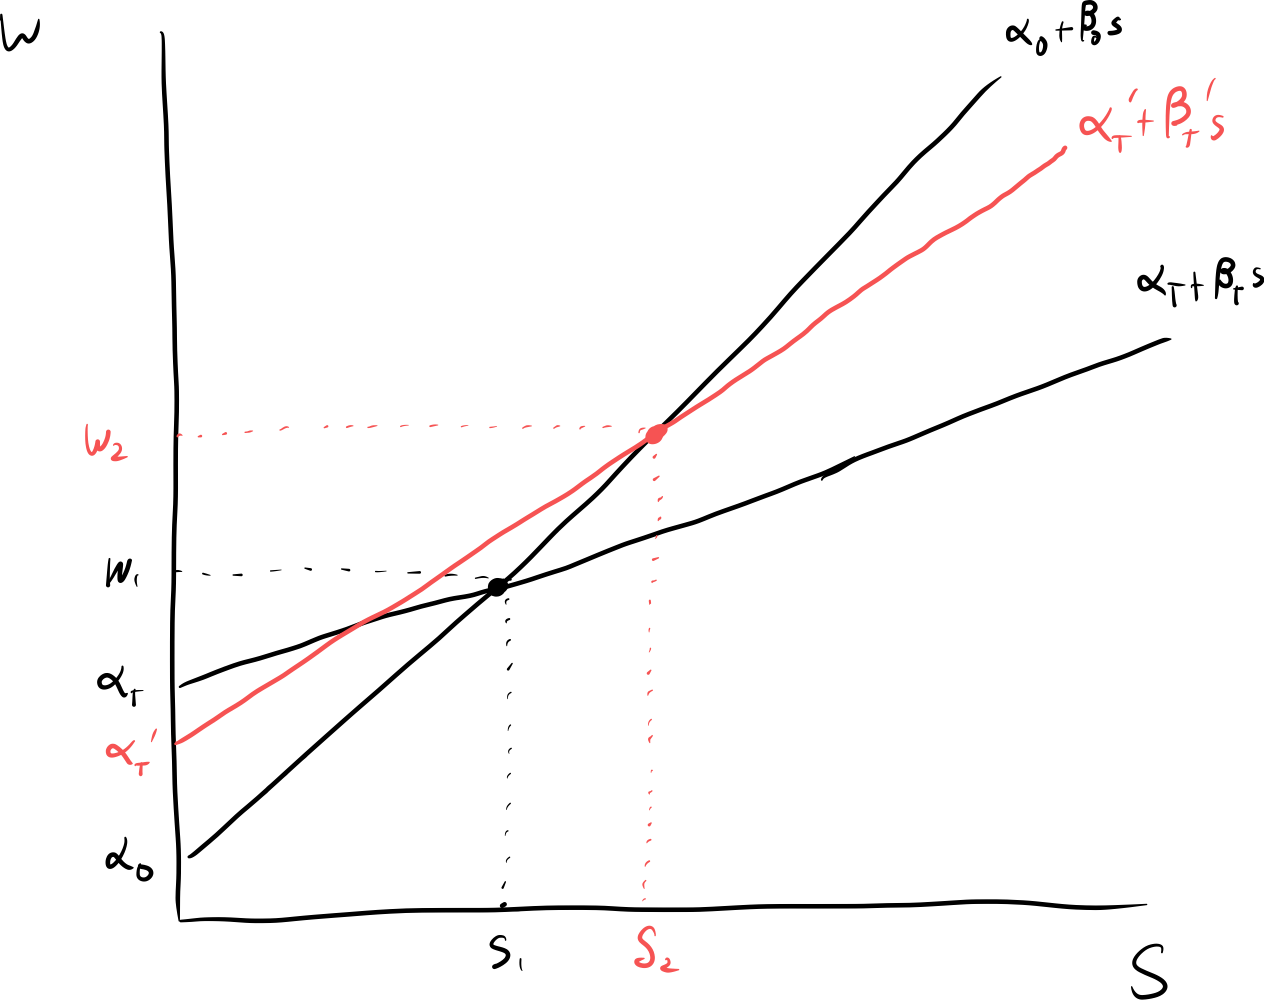
\includegraphics[width=10cm]{images/ps3q3c.png}
      \end{center}
    \item The crash in the stock market reduces the returns to skill and the endowment in outside options, meaning that the skill and wage of teachers increases.
      \begin{center}
        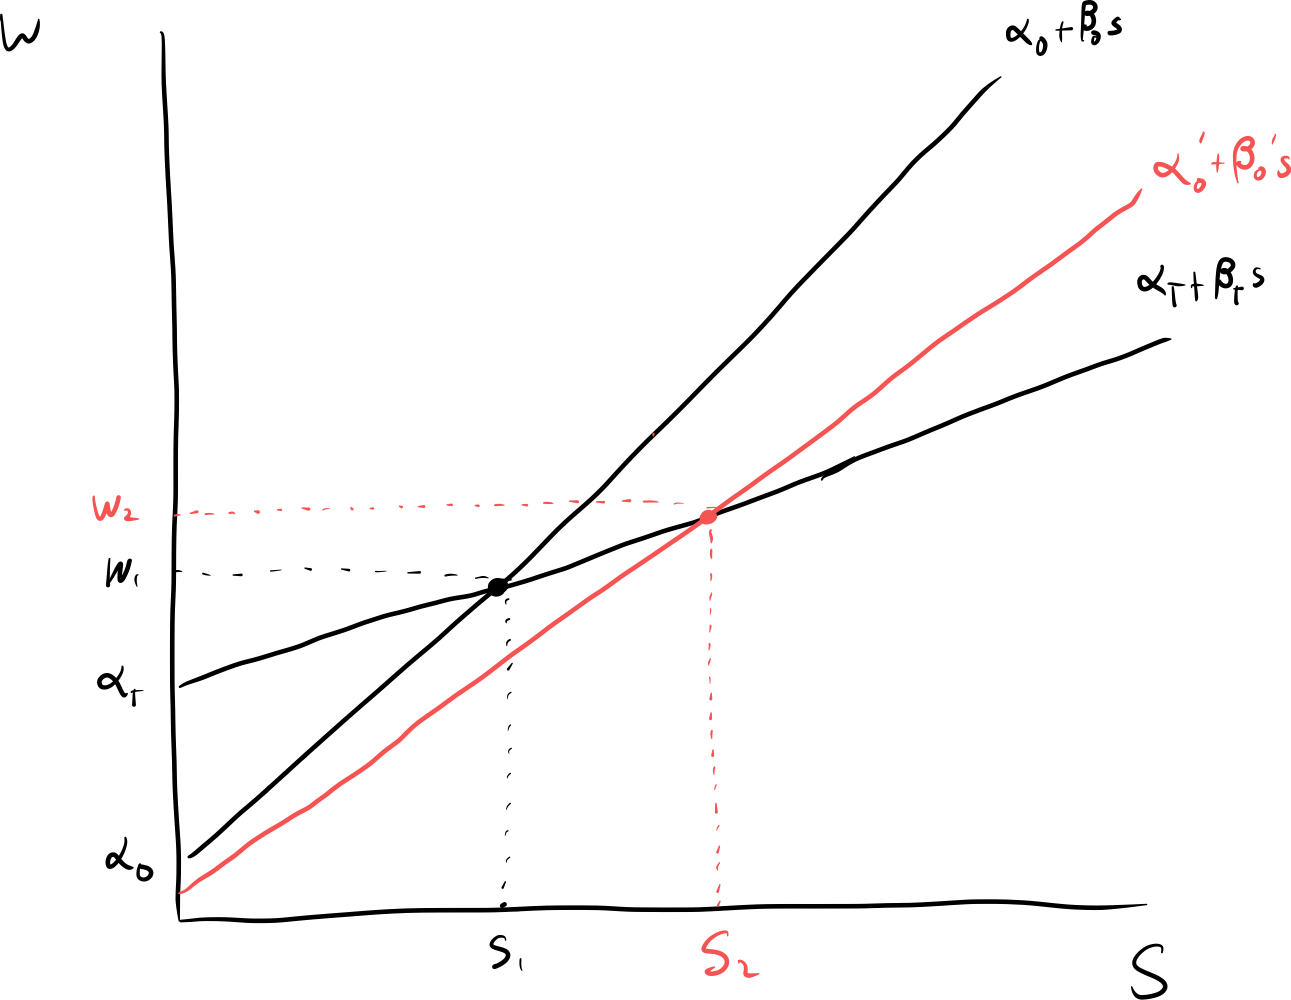
\includegraphics[width=10cm]{images/ps3q3d.png}
      \end{center}
    \item Teach for America increases the return to skill for teachers, leading to higher skill and wage levels.
      \begin{center}
        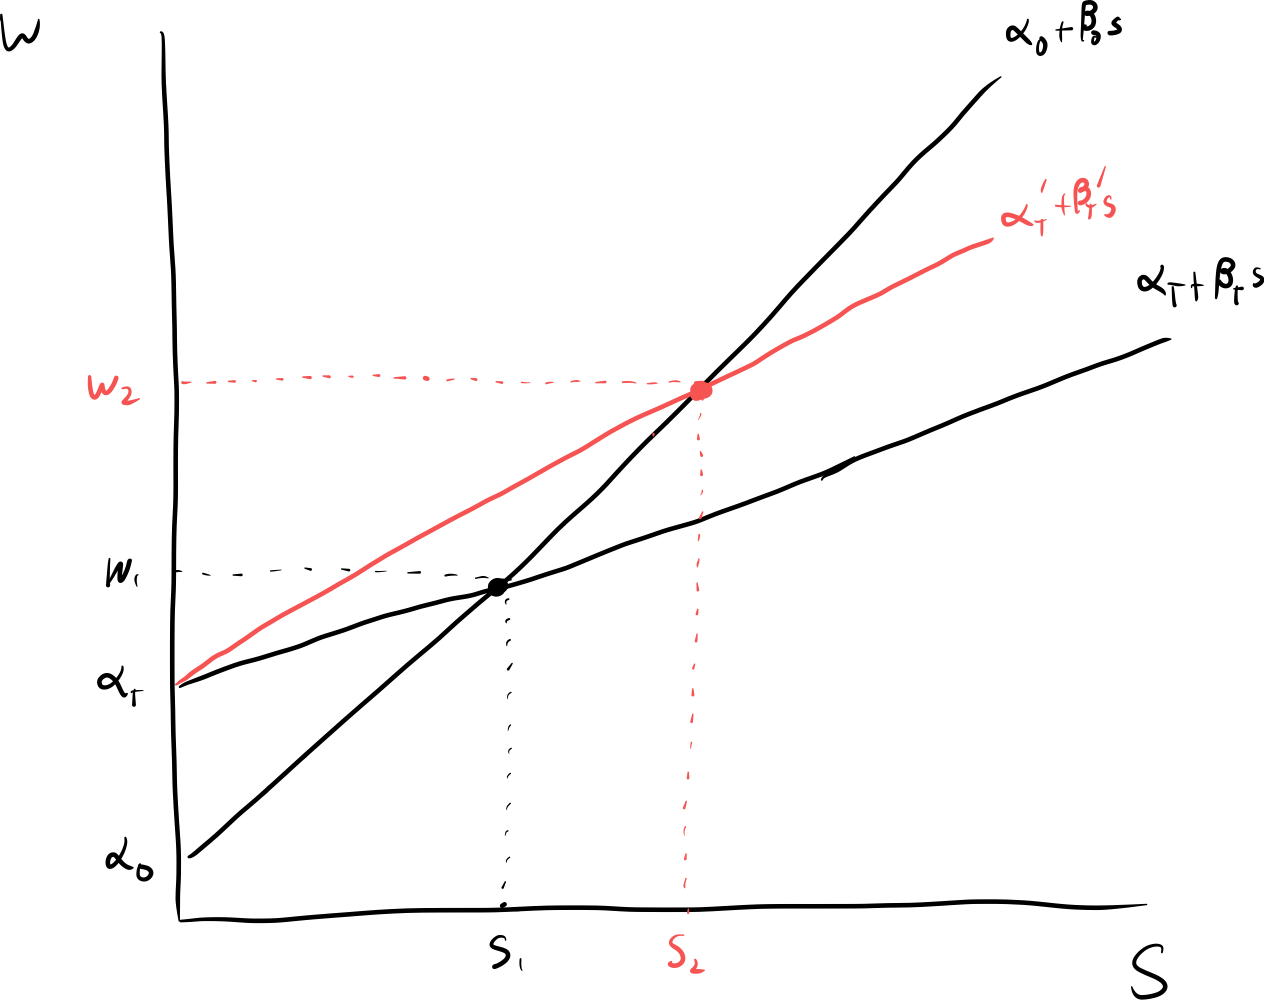
\includegraphics[width=10cm]{images/ps3q3e.png}
      \end{center}
  \end{enumerate}
  \section{School Accountability}%
  \subsection{Problem 4}%
  The No Child Left Behind act mandated that states implement measures of reward and punishment on the basis of performance of schools in standardized tests in reading and mathematics. Specifically, qua Dee and Jacob's description, NCLB mandated sanctions such as staff dissolution and school restructuring for schools that were recipients of funds from Title I of the ESEA that failed to meet adequate yearly progress goals. The primary intent of NCLB was to improve outcomes for low-performing schools by aligning incentives for education with measurable targets of performance and progress.
  \subsection{Problem 5}%
  \begin{enumerate}[(a)]
    \item My elementary school's academic progress was rated as an 8/10, with test scores well above the state average --- the school had 93\% proficiency in math, compared to the state average of 35\%, 91\% proficiency in English, compared to the state average of 47\%, and 88\% proficiency in science, compared to the state average of 30\%.\\

      The only subgroup that was tested was Asians (as the school is 88\% Asian), and were around the same level of proficiency as the general population of the school.
    \item The school was 4\% White, 3\% Hispanic, 88\% Asian, and 1\% African-American. 8\% of students receive free or reduced-price lunch, and 9\% are English language learners. It is likely that the ratings overestimate the quality of education at the school, due to the particularly unrepresentative demographics of students.
    \item California could better normalize for student demographics (especially on the basis of income) so as to better reflect a tabula rasa-esque approach towards receiving education at the school. However, it is quite difficult to normalize on the basis of demographics in a school with a particularly unrepresentative student body.
    \item Based on the test scores, I would probably send my children to the elementary school since it evidently has a very high level of proficiency among its students. How much of that is peer effects vs. teacher quality is hard to determine, however.
  \end{enumerate}
  \subsection{Problem 6}%
  \begin{enumerate}[(a)]
    \item The average score in teacher $i$'s class in any given year is influenced by a multitude of factors outside of teacher $i$'s control, and thus assigning accountability measures on the basis of random variation would be quite detrimental. However, at the same time, this methodology is also one of the simplest measures to implement.
    \item Similarly to using average test score, a cutoff metric would be subject to idiosyncratic variation that would assign punishment or reward without basis in the teacher's quality itself. However, similar to using average test scores, this metric would be one of the simplest measures to implement.
    \item This would likely be the most effective measure of teacher value add, as it effectively extracts the effect of the teacher on the students' test performance. However, at the same time, harmonizing such data would be costly.
    \item This measure would be easier to implement than the previous measure, as it measures changes in test scores for a given year, but also is not a true measure of value-add, as changes in test scores are still subject to idiosyncratic variation from year to year.
  \end{enumerate}
\end{document}
